
% Requires: \usepackage{tikz}
% Simple TikZ version (more manual but widely compatible)

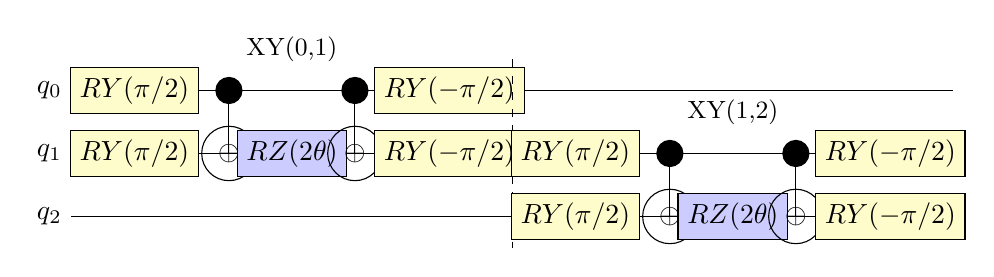
\begin{tikzpicture}[scale=0.8]
    % Define coordinates
    \foreach \i in {0,1,2} {
        \draw (0,2-\i) -- (14,2-\i);
        \node[left] at (0,2-\i) {$q_{\i}$};
    }
    
    % XY Interaction (0,1)
    \node[draw, fill=yellow!20] at (1,2) {$RY(\pi/2)$};
    \node[draw, fill=yellow!20] at (1,1) {$RY(\pi/2)$};
    
    \node[draw, circle, fill=black] at (2.5,2) {};
    \draw (2.5,2) -- (2.5,1);
    \node[draw, circle, minimum size=0.3cm] at (2.5,1) {$\oplus$};
    
    \node[draw, fill=blue!20] at (3.5,1) {$RZ(2\theta)$};
    
    \node[draw, circle, fill=black] at (4.5,2) {};
    \draw (4.5,2) -- (4.5,1);
    \node[draw, circle, minimum size=0.3cm] at (4.5,1) {$\oplus$};
    
    \node[draw, fill=yellow!20] at (6,2) {$RY(-\pi/2)$};
    \node[draw, fill=yellow!20] at (6,1) {$RY(-\pi/2)$};
    
    % Barrier
    \draw[dashed] (7,2.5) -- (7,-0.5);
    
    % XY Interaction (1,2)
    \node[draw, fill=yellow!20] at (8,1) {$RY(\pi/2)$};
    \node[draw, fill=yellow!20] at (8,0) {$RY(\pi/2)$};
    
    \node[draw, circle, fill=black] at (9.5,1) {};
    \draw (9.5,1) -- (9.5,0);
    \node[draw, circle, minimum size=0.3cm] at (9.5,0) {$\oplus$};
    
    \node[draw, fill=blue!20] at (10.5,0) {$RZ(2\theta)$};
    
    \node[draw, circle, fill=black] at (11.5,1) {};
    \draw (11.5,1) -- (11.5,0);
    \node[draw, circle, minimum size=0.3cm] at (11.5,0) {$\oplus$};
    
    \node[draw, fill=yellow!20] at (13,1) {$RY(-\pi/2)$};
    \node[draw, fill=yellow!20] at (13,0) {$RY(-\pi/2)$};
    
    % Labels
    \node[above] at (3.5,2.3) {\small XY(0,1)};
    \node[above] at (10.5,1.3) {\small XY(1,2)};
\end{tikzpicture}
